
\begin{frame}
\frametitle{Coral Reef}
\begin{itemize}
\item A complex aquatic ecosystem physically supported by calcium carbonate secretions of the colorful stone coral. \\
\item Modeling approach by Li-Wang-Zhang-Hastings is to describe the relationships between macroalgae, algal turfs, and corals (Li et al., 2014).
\end{itemize}
\end{frame}

\begin{frame}
\frametitle{Coral Reef Ecosystem} McClanahan identifies three major component:
\begin{itemize}
\item primary producers (coral and algae)\\
\item herbivores (e.g. parrotfish)\\
\item carnivores (McClanahan, 1994).
\end{itemize}
\end{frame}

\begin{frame}
\frametitle{Coral Reef Dynamics}
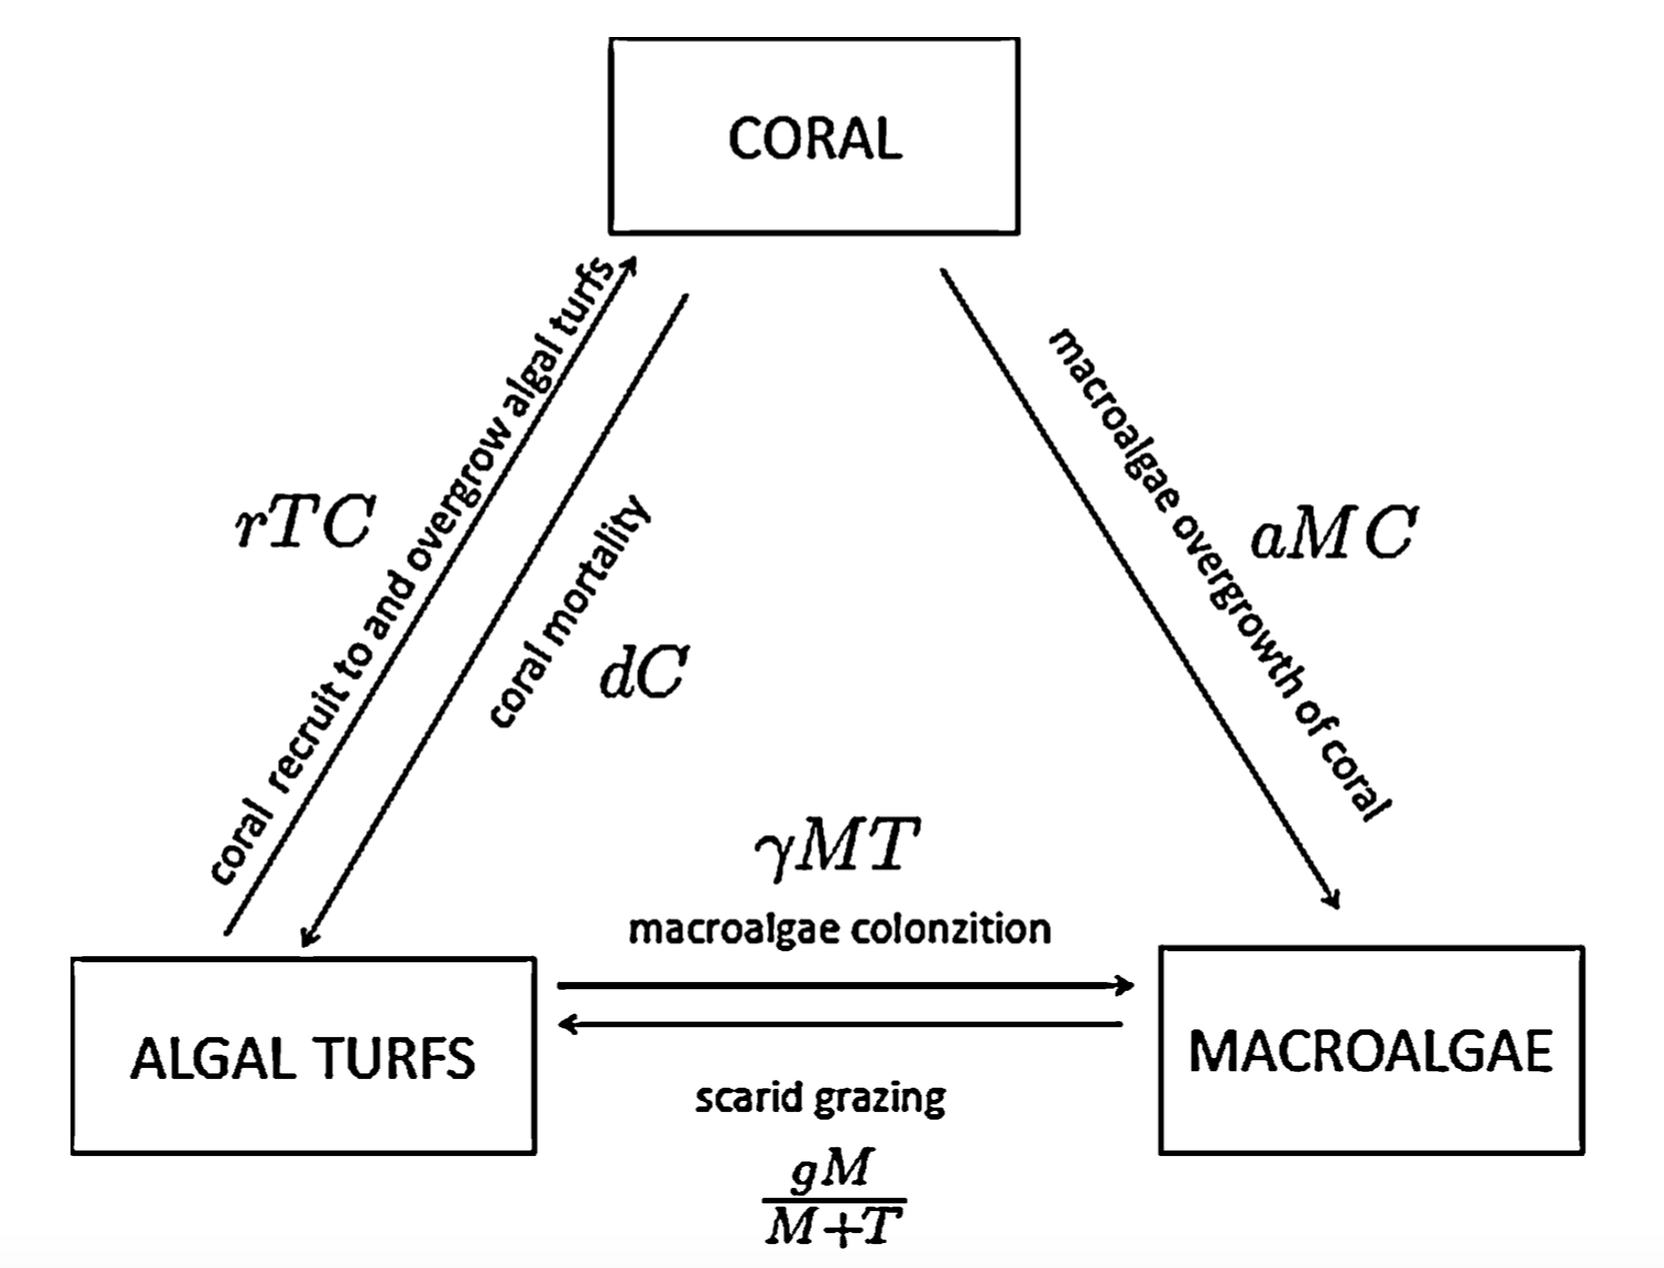
\includegraphics[scale=.175]{./coral-reef-triangle.png}
\end{frame}

\begin{frame}\frametitle{Coral Reef Dynamics}
The ordinary differential equation model:
$$\begin{cases}\begin{array}{rl}
\frac{dM}{dt}\hspace{-.8em}&=aMC - \frac{gM}{M+T} + \gamma M T\\
\frac{dC}{dt}\hspace{-.8em}&=rTC - dC - aMC\\
\frac{dT}{dt}\hspace{-.8em}&=\frac{gM}{M + T} - \gamma MT - rTC + dC
\end{array}\end{cases},$$ where \begin{itemize}\itemsep0pt
\item $r$ is the rate corals overgrow upon algal turfs\\
\item $d$ is the mortality rate of corals\\
\item $a$ is the rate that macroalgae overgrow upon corals\\
\item $\gamma$ is the rate that macroalgae spread over algal turfs\\
\item $g$ is the indiscriminate grazing rate of parrotfish.
\end{itemize}
\end{frame}

\begin{frame}\frametitle{Coral Reef Dynamics}
\hspace{1.57em}\begin{itemize}
\item \frac{dT}{dt}=-\frac{dM}{dt}-\frac{dC}{dt}$ implies $M+C+T$ is constant, say $M+C+T=1$.
\item This limits our scope to regions entirely covered by coral, macroalgae, and algal turf. \end{itemize}
Thus we reduce our system to, $$\begin{cases}
\begin{array}{rl}
\frac{dM}{dt}&= aMC-\frac{gM}{1-C} + \gamma M - \gamma M^2 -\gamma M C\\
\frac{dC}{dt}&=rC - rC^2 - rCM - dC - aMC
\end{array} \end{cases}.$$
\end{frame}

\begin{frame}
\frametitle{Time Delay in the Coral Ecosystem}
We can identify time delays in the coral ecosystem:
\begin{itemize}
\item the delay between the grazing of macroalgae and growth of algal turf (Li et al., 2014).\\
\item  the delay between the growth of algae and the effect of algae on coral (Jompa, 2003).
\end{itemize}
\end{frame}

\begin{frame}\frametitle{Coral Reef Dynamics}
Delay Differential Equation Model:
$$\begin{cases}\begin{array}{rl}
\frac{dM}{dt}\hspace{-.8em}&=aMC - \frac{gM(t-\tau)}{1-C(t-\tau)}+\gamma M T\\
\frac{dC}{dt}\hspace{-.8em}&=rTC - dC - aMC\\
\end{array}\end{cases}.$$
\end{frame}

\begin{frame}
\frametitle{Equilibria and Stability}
\end{frame}

\begin{frame}
\frametitle{Stochastic Model}
Let's add noise!
$$\begin{cases}\begin{array}{rl}
\frac{dM}{dt}\hspace{-.8em}&=aMC - \frac{gM(t-\tau)}{1-C(t-\tau)}+\gamma M T+\beta M(1-M)dW\\
\frac{dC}{dt}\hspace{-.8em}&=rTC - dC - aMC\\
\end{array}\end{cases}.$$
\end{frame}
